\documentclass[journal,12pt,twocolumn]{IEEEtran}

\usepackage{setspace}
\usepackage{gensymb}
\singlespacing
\usepackage[cmex10]{amsmath}

\usepackage{amsthm}

\usepackage{mathrsfs}
\usepackage{txfonts}
\usepackage{stfloats}
\usepackage{bm}
\usepackage{cite}
\usepackage{cases}
\usepackage{subfig}

\usepackage{longtable}
\usepackage{multirow}

\usepackage{enumitem}
\usepackage{mathtools}
\usepackage{steinmetz}
\usepackage{tikz}
\usepackage{circuitikz}
\usepackage{verbatim}
\usepackage{tfrupee}
\usepackage[breaklinks=true]{hyperref}
\usepackage{graphicx}
\usepackage{tkz-euclide}

\usetikzlibrary{calc,math}
\usepackage{listings}
    \usepackage{color}                                            %%
    \usepackage{array}                                            %%
    \usepackage{longtable}                                        %%
    \usepackage{calc}                                             %%
    \usepackage{multirow}                                         %%
    \usepackage{hhline}                                           %%
    \usepackage{ifthen}                                           %%
    \usepackage{lscape}     
\usepackage{multicol}
\usepackage{chngcntr}

\DeclareMathOperator*{\Res}{Res}

\renewcommand\thesection{\arabic{section}}
\renewcommand\thesubsection{\thesection.\arabic{subsection}}
\renewcommand\thesubsubsection{\thesubsection.\arabic{subsubsection}}

\renewcommand\thesectiondis{\arabic{section}}
\renewcommand\thesubsectiondis{\thesectiondis.\arabic{subsection}}
\renewcommand\thesubsubsectiondis{\thesubsectiondis.\arabic{subsubsection}}


\hyphenation{op-tical net-works semi-conduc-tor}
\def\inputGnumericTable{}                                 %%

\lstset{
%language=C,
frame=single, 
breaklines=true,
columns=fullflexible
}
\begin{document}

\newcommand{\BEQA}{\begin{eqnarray}}
\newcommand{\EEQA}{\end{eqnarray}}
\newcommand{\define}{\stackrel{\triangle}{=}}
\bibliographystyle{IEEEtran}
\raggedbottom
\setlength{\parindent}{0pt}
\providecommand{\mbf}{\mathbf}
\providecommand{\pr}[1]{\ensuremath{\Pr\left(#1\right)}}
\providecommand{\qfunc}[1]{\ensuremath{Q\left(#1\right)}}
\providecommand{\sbrak}[1]{\ensuremath{{}\left[#1\right]}}
\providecommand{\lsbrak}[1]{\ensuremath{{}\left[#1\right.}}
\providecommand{\rsbrak}[1]{\ensuremath{{}\left.#1\right]}}
\providecommand{\brak}[1]{\ensuremath{\left(#1\right)}}
\providecommand{\lbrak}[1]{\ensuremath{\left(#1\right.}}
\providecommand{\rbrak}[1]{\ensuremath{\left.#1\right)}}
\providecommand{\cbrak}[1]{\ensuremath{\left\{#1\right\}}}
\providecommand{\lcbrak}[1]{\ensuremath{\left\{#1\right.}}
\providecommand{\rcbrak}[1]{\ensuremath{\left.#1\right\}}}
\theoremstyle{remark}
\newtheorem{rem}{Remark}
\newcommand{\sgn}{\mathop{\mathrm{sgn}}}
\providecommand{\abs}[1]{\vert#1\vert}
\providecommand{\res}[1]{\Res\displaylimits_{#1}} 
\providecommand{\norm}[1]{\lVert#1\rVert}
%\providecommand{\norm}[1]{\lVert#1\rVert}
\providecommand{\mtx}[1]{\mathbf{#1}}
\providecommand{\mean}[1]{E[ #1 ]}
\providecommand{\fourier}{\overset{\mathcal{F}}{ \rightleftharpoons}}
%\providecommand{\hilbert}{\overset{\mathcal{H}}{ \rightleftharpoons}}
\providecommand{\system}{\overset{\mathcal{H}}{ \longleftrightarrow}}
	%\newcommand{\solution}[2]{\textbf{Solution:}{#1}}
\newcommand{\solution}{\noindent \textbf{Solution: }}
\newcommand{\cosec}{\,\text{cosec}\,}
\providecommand{\dec}[2]{\ensuremath{\overset{#1}{\underset{#2}{\gtrless}}}}
\newcommand{\myvec}[1]{\ensuremath{\begin{pmatrix}#1\end{pmatrix}}}
\newcommand{\mydet}[1]{\ensuremath{\begin{vmatrix}#1\end{vmatrix}}}
\numberwithin{equation}{subsection}
\makeatletter
\@addtoreset{figure}{problem}
\makeatother
\let\StandardTheFigure\thefigure
\let\vec\mathbf
\renewcommand{\thefigure}{\theproblem}
\def\putbox#1#2#3{\makebox[0in][l]{\makebox[#1][l]{}\raisebox{\baselineskip}[0in][0in]{\raisebox{#2}[0in][0in]{#3}}}}
     \def\rightbox#1{\makebox[0in][r]{#1}}
     \def\centbox#1{\makebox[0in]{#1}}
     \def\topbox#1{\raisebox{-\baselineskip}[0in][0in]{#1}}
     \def\midbox#1{\raisebox{-0.5\baselineskip}[0in][0in]{#1}}
\vspace{3cm}
\title{AI1103-Assignment 5}
\author{Name : Ayush Jha \\ Roll Number: CS20BTECH11006}
\maketitle
\newpage
\bigskip
\renewcommand{\thefigure}{\theenumi}
\renewcommand{\thetable}{\theenumi}
Download all python codes from 
\begin{lstlisting}
https://github.com/ayushjha2612/AI11003/tree/main/Assignment5/Codes
\end{lstlisting}
%
and latex-tikz codes from 
%
\begin{lstlisting}
https://github.com/ayushjha2612/AI11003/tree/main/Assignment5
\end{lstlisting}
\section{GATE 2020 XE-A Q.11}
Players A and B take turns to throw a fair dice with six faces. If A is the first player to throw, then the probability of B being the first one to get a six is --- ( round of to two decimal places). \\

\section{Answer}
0.45
\section{Solution}
Let the random variable X represent which player gets six first. That is $X=0 $ when A gets a six first and $X=1 $ when B gets six first. \\
Let another random variable Y represent getting a six on the dice. $Y=1 $ for six and $Y=0 $ for any other number. \\
\begin{align}
    \Pr\brak{Y=0} = \frac{5}{6} \\
    \Pr\brak{Y=1} = \frac{1}{6}
\end{align}
\textbf{Case 1} : \\
A does not get six and B does in the first turn i.e. 
\begin{align}
    X&=1  \\
    \Pr\brak{X=1} &= \Pr_{A}\brak{Y=0} \times \Pr_{B}\brak{Y=1} \\
        &= \frac{5}{36}
\end{align}

\textbf{Case 2} : \\
A does not get six and B does in the second turn i.e. 
\begin{align}
    \Pr\brak{X=1} &= {\Pr\brak{Y=0}}^3  \times \Pr\brak{Y=1} \\
              &= \frac{5^3}{36^2}
\end{align}
\textbf{Case 3} : \\
A does not get six and B does in the third turn i.e. 
\begin{align}
    \Pr\brak{X=1} &= {\Pr\brak{Y=0}}^5  \times \Pr\brak{Y=1} \\
              &= \frac{5^5}{36^3}
\end{align}
And so on $\hdots$ \\
The further cases have been summarized in table \ref{tab:Cases} \\
\begin{table}[hbt]
\centering
\begin{tabular}{|c|c|c|}
\hline
\textbf{Case}          & \textbf{No. of turns} & \textbf{Probability}  \\ \hline
4                      & 4                     & $5^7/36^4$             \\ \hline
5                      & 5                     & $ 5^9 / 36 ^5 $        \\ \hline
$\vdots$               & $\vdots$             & $\vdots$               \\
n                      & n                     & $5^{2n-1}/6^{2n} $      \\ \hline
\vdots                 & \vdots                & \vdots                  \\ \hline
\end{tabular}
\caption{Generalization of cases}
\label{tab:Cases}
\end{table}

Thus the total probability is sum of these individual probabilities i.e.
\begin{align}
    \Pr\brak{X=0} &= \frac{5}{6^2} + \frac{5^3}{6^4} + \hdots + \frac{5^{2n-1}}{6^{2n}} +\hdots  \\
    &= \frac{5}{6^2} \times \brak{1 + \frac{5^2}{6^2} + \frac{5^4}{6^4} + \hdots } 
\end{align}
By Using sum of infinite GP we have, 
\begin{align}
     \Pr\brak{X=0} &= \frac{5}{6^2} \times \brak{\frac{1}{1 - \frac{25}{36}}}  \\
       &= \frac{5}{36} \times \frac{36}{11} \\
       &= \frac{5}{11} = 0.45
\end{align}
Therefore the probability of B being the first one to get a six is $ 0.45 $.\\
The theory vs Simulation plot can be seen at figure \ref{fig::Probability distribution}.
\begin{figure}[h!]
    \centering
    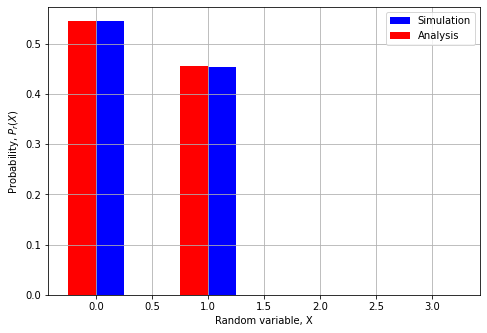
\includegraphics[width=.9\columnwidth]{Assignment_5.png}
    \caption{Probability distribution of X}
    \label{fig::Probability distribution}
\end{figure}
\end{document}